\section{Example Instances}


In order to visualize the problem and attack it using more intuition, we must consider that the cuts at integer points can 
be seen easily in the following manner. Given a graph G and an ordering function f, we draw the nodes in an horizontal line, in the order given by f. What we are trying to minimize is the size maximum cut among the $S_i$'s , where $S_i=\{v \in V : f(v) \leq i\}$, for $i=1,2,\ldots,n-1$. But on the graph drawing mentioned above, the size of every $S_i$ is the number of edges existing in the space between the vertical lines passing by nodes i and i+1. To give an example, in the following linear
arrangement we easily deduce that the minimum $S_i$ size is 3:


\begin{center}
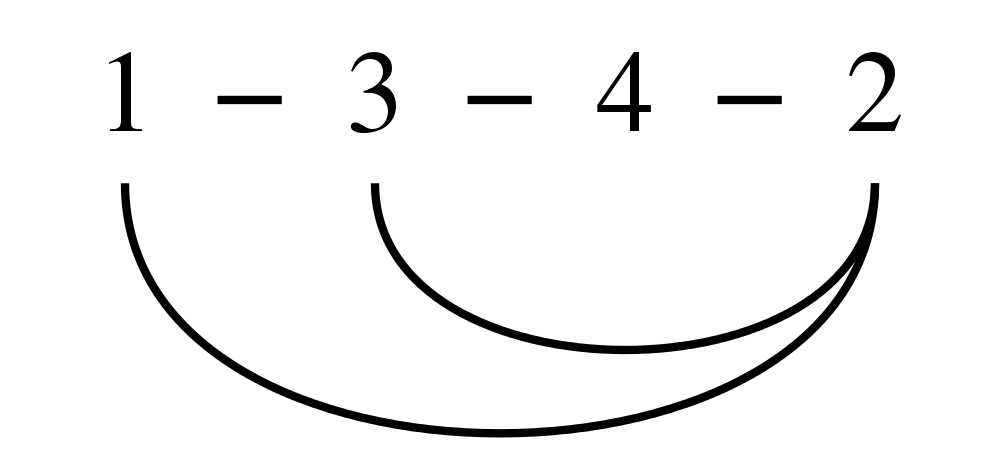
\includegraphics[height=2.5cm,width=6cm]{img/graph2.png}
\end{center}

\textbf{TODO: draw another example}

The problem instances are Graphs G. As an example, we take $G=K_5$:


\begin{center}
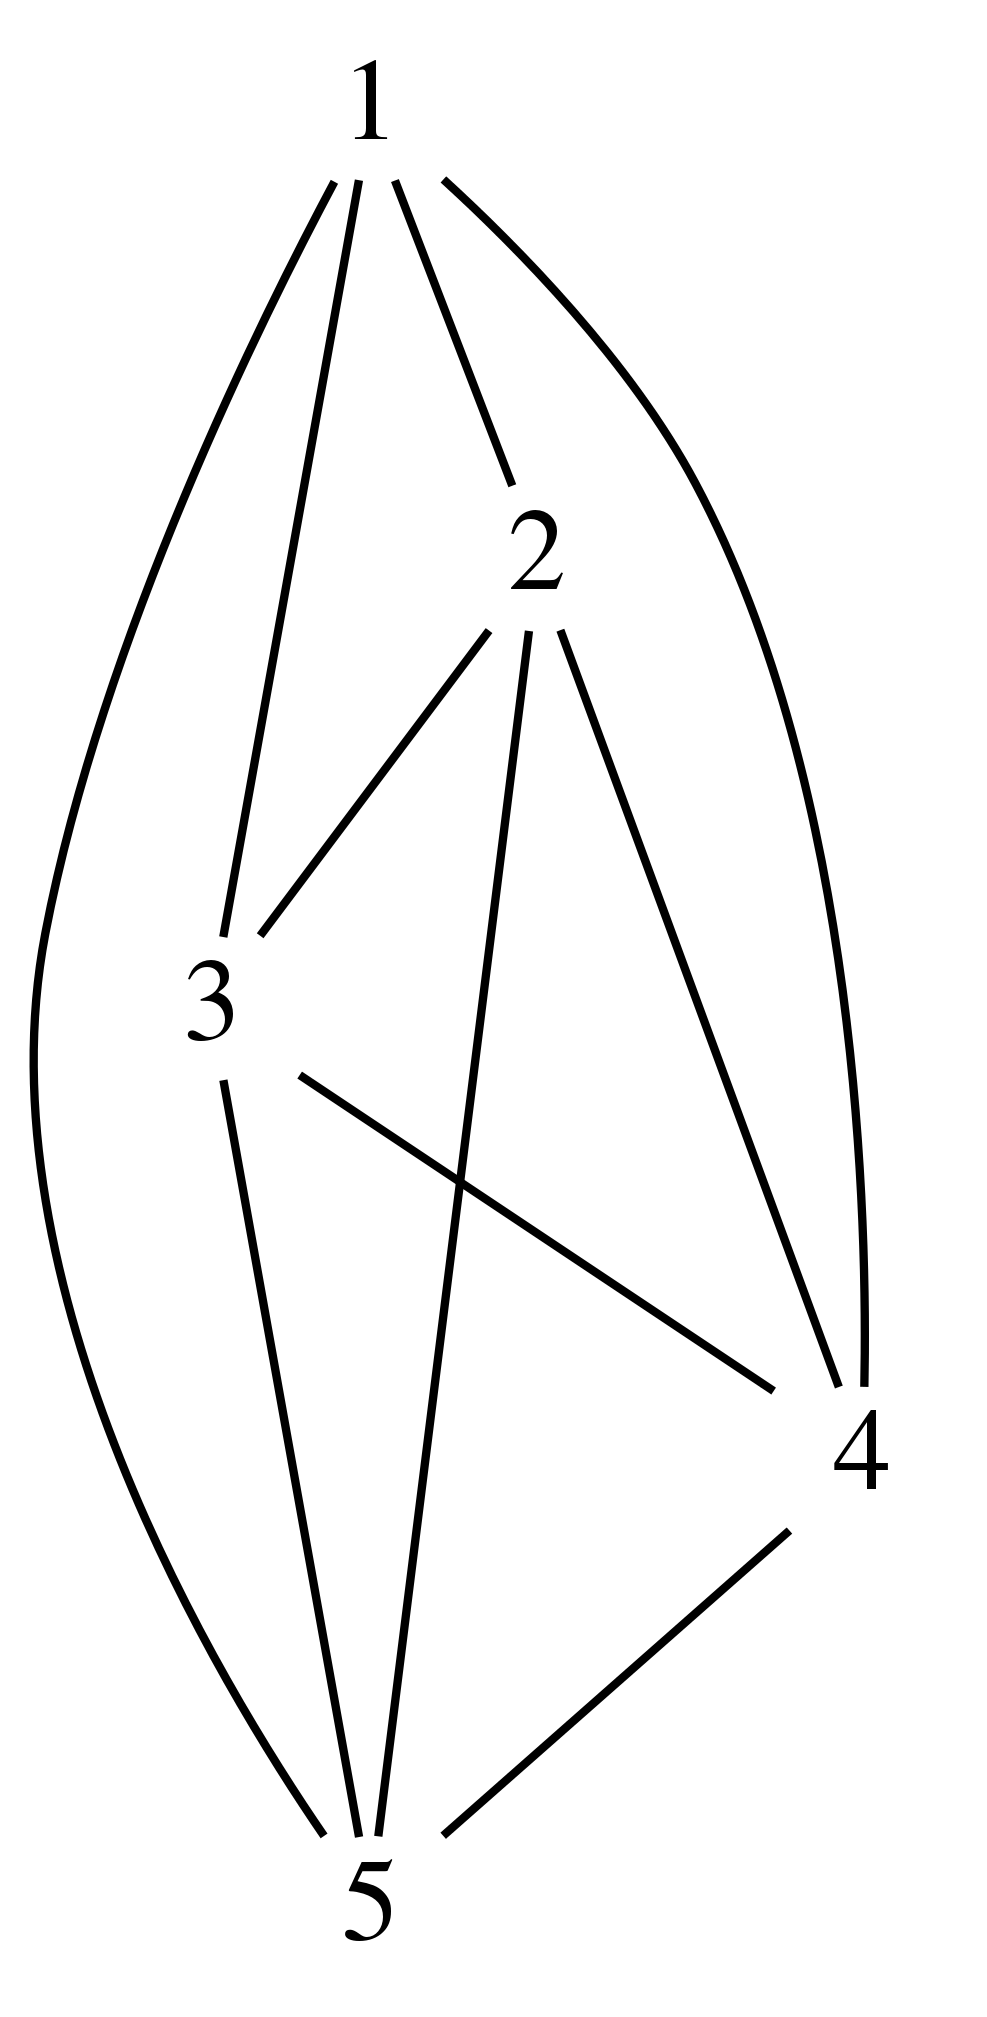
\includegraphics[scale=0.1]{img/k5.png}
\end{center}



Here, every node is connected to every one of the rest. Therefore, every node is identical to every one else. In this case, 
every assignment of numbers $1\ldots n$ to the nodes yields the same graph. Therefore to solve this instance, we consider a random labeling of our nodes, and we compute the cuts at all integer points between 1 and n. 


Another instance, could be this graph.

\begin{center}
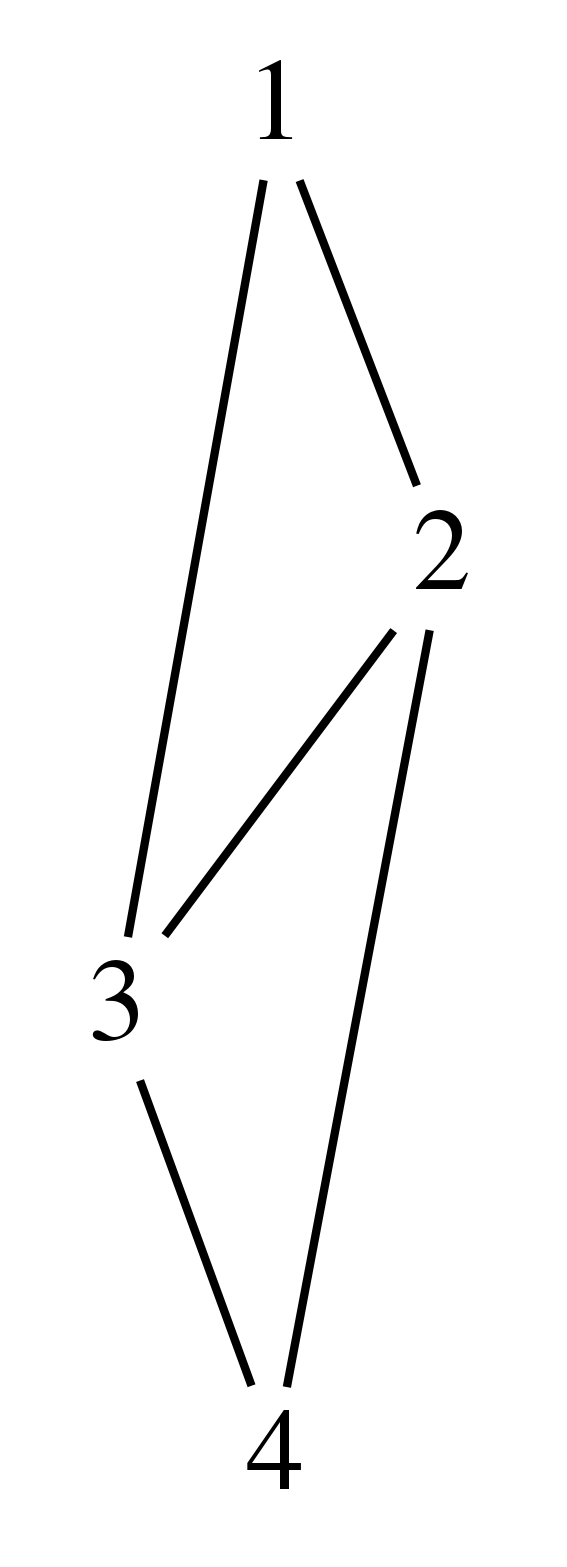
\includegraphics[scale=0.1]{img/graph3.png}
\end{center}


Here, the assignment matters. In order to attack the problem in a more intuitive manner, it would be more suitable to have visualize the problem as follows: Given graph G, create a drawing of G such that the nodes are placed on a straight horizontal line.
The objective is to minimize the maximum number of edges that exist in the space between two consecutive nodes. 
For example, the graph below is a visualization of the assignment $f(1)=1, f(2)=4,f(3)=2,f(4)=3$, which gives us $max(S_i)=3$.

\begin{center}
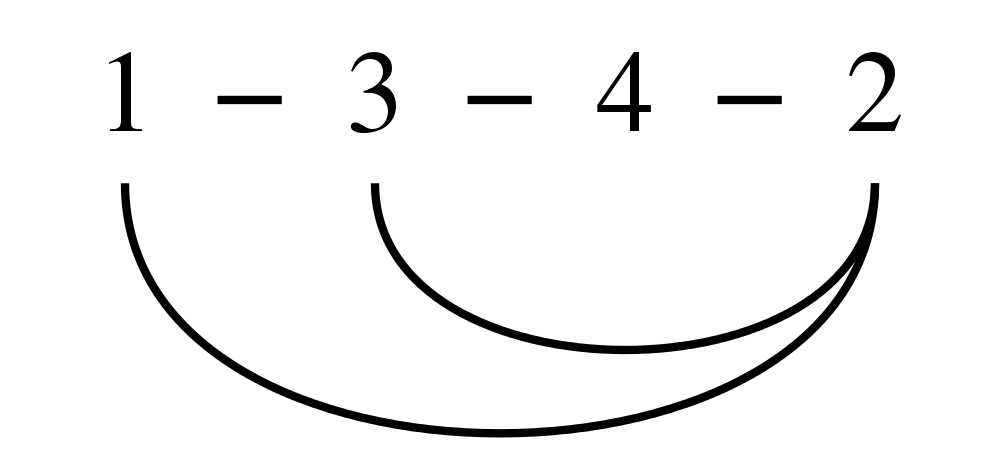
\includegraphics[scale=0.1]{img/graph2.png}
\end{center}

By the way, the above assignment gives us the best possible results, w.r.t. the requirements of the problems. That is, there is no assingment that gives us a lower maximum cutwidth. \textbf{explain better here}


